%!TEX root = ../main.tex

\documentclass[../main.tex]{subfiles} 
\begin{document}

\section{Simulation Study}\label{sec:simulation_study}
The previous section shows how the model presented in this thesis can be useful in the identification of changes in relative skill prices in panel data. Following this identification strategy, changes in the prices of skills can be determined on the basis of the realized wages and task choices. In this section, I provide an exemplary application of this identification in the format of a simulation study.\footnote{Program codes of this simulation study are available on GitHub: github.com/DaLueke/estimating\_skill\_prices.}
\\
As part of this simulation study I, first, generate a representation of a panel data set. The data generating process endogenously provides optimal task choices and according realized wages for each simulation period on the basis of potential task specific wages. For each task the potential wages are composed of exogenous skill prices as well as  skill endowments that are exogenous in the initial period and evolve endogenously based on optimal task choices in subsequent periods.
\\
In a second step, I rely on this simulated data for an estimation of changes in relative skill prices following the identification strategy presented in section \ref{sec:tractable-model-of-cont-task-choice} of this thesis. This involves an estimation of skill accumulation and changes in amenities in a base period. Subsequently, these estimated are used to isolate effects of changes in skill prices from skill accumulation and changes in amenities in the following period. After this preliminary step, adjusted wage changes are used to estimate changes in relative skill prices.

\subsection{Data Generating Process} \label{sec:DGP}
% Generate 3 points in time so that I observe two intertemporal changes
%% Split into base period and a subsequent estimation period
% Generate potential wages
%% Skill prices: Exogeneously given. Constant in base period, changing in estimation period
%% Skill Endowments: Exogenous starting values, skill accumulation afterwards
%% Learning by doing process: Workers become better at the task they are doing relatively much.
% Penalty term: generate exogenous preferences for a task split
% Obtain optimally chosen task choice parameters by maximizing wages minus penalty
% Determine wage that results from optimal choice of tasks
% Can I find some nice way of visualizing my simulated data?
In order to produce a representation of a panel data set, the data generating process provides data on three points in time so that two inter temporal changes can be calculated. The first thereof serves as a base period and the second as an estimation period. Following the discussion of the model in section \ref{sec:implications-with-j=2}, this simulation is based on two different tasks. With the objective of simulating a utility maximization process in mind, both wages and penalty term need to be simulated (see equation \ref{eq:utility}). Therefore, I first describe the data generating process for potential task specific wages. Second, I present the parameterization of the penalty term.
\\
The wage function depends on task specific potential wages, which are assumed to result as sum of respective skill prices and individual skill endowments (see section \ref{sec:identifying-changes-in-skill-prices}, particularly equation (\ref{eq:potential_wages})). Prices of each skill in each period are exogenous to the data generating process. In this simulation study specifically, relative skill prices are set to be constant during the base period and changing during the estimation period. In order to facilitate the evaluation of estimation results, the change of relative skill prices in the estimation period is deterministic.
\\
Initial values of skill endowments are exogenous to the data generating process and, thus, are drawn from a normal distribution. In subsequent periods, skills endowments experience an accumulation that is modeled as a learning by doing process. In particular, workers gain relative skill in that task, which they execute to a relatively large extent. The stronger a worker focuses on one single task, the larger is the gain in relative skill herein. This results in an endogenous skill accumulation that depends on task choices. The particular functional form of skill accumulation is presented in equation (\ref{eq:skill_accumulation}).
\begin{equation} \label{eq:skill_accumulation}
\tilde{s}_{i,t} = \tilde{s}_{i, t-1} + (\lambda_{i, t-1}^* - 0.5)
\end{equation}
In accordance to the normalization of potential wages introduced in section \ref{sec:implications-with-j=2}, potential wages of task one are normalized to zero so that potential wages of task two need to be understood as relative sizes. Specifically, a skill endowment for task two that is positive indicates that a worker has a comparative advantage in executing this task and vice versa for negative skill endowments. Analogously, a relative skill price that is larger than zero implies a higher compensation for executing task two than for task one.
\\
The penalty term is a function of individual time allocation preference, which is captured in parameter $b_i$. For this simulation study this parameter is generally assumed to be uniformly distributed within some borders $\{b_{low}, b_{high}\}$ with $b_{low}, b_{high} \in [0, 1] \; \text{and} \; b_{low} \leq b_{high}$. The resulting interval is assumed to be centered at the equal split of working time on both tasks, so that neither task is systematically preferred to the other. Additionally, it is assumed that workers dislike strong specialization (section \ref{sec:utility-max-problem}). To do justice to this assumption, the limits of the parameter for preferred allocations should, therefore, not be chosen in the extremes. In the data generated process that is used for the simulation study, the borders of individual time allocation preferences are set to $b_{low} = 0.3$ and $b_{high} = 0.7$.
\\
For this simulation study, I use a quadratic specification of the penalty function, i.e. the penalty exponent is set to $\phi = 2$. This specification meets  the assumed properties of the penalty function. At the same time, it results optimal task choices that are a linear function in relative potential wages, which makes the linear interpolation of inter temporal changes in task choices an exact solution. The penalty weight parameter is set to a value of $\theta = 15$ in this data generating process. This weight is chosen so that neither realized wages nor the penalty dominates the utility function. While the first case could result in a large number of corner solutions where every worker focuses on the task with higher potential wage, the second case would produce a dataset in which workers mostly stick with their preferred task choice so that potential wages, and more importantly changes thereof, impact task choice very little. Based on both, potential wages and the penalty term, the optimal task choice parameter $\lambda_{i,t}^*$ can be obtained in each period by maximizing the individual utility (i.e., realized wage lessened by the penalty term). Furthermore, resulting realized wages can be calculated using this optimal task choice.
\\
A representation of the simulated data can be seen in figure \ref{fig:simulated_data}. Particularly, the figure shows the combinations of optimal task choices $\lambda_{i,t=0}^*$ and realized wages $w_{i,t=0}$ for all $N=100$ simulated workers in the initial period from one of the Monte Carlo iterations. From the graphic it can be seen that task choices (horizontal axis) are distributed around the equal split, with no worker engaging in an complete specialization on either one of the tasks. The histogram of realized relative wages (vertical axis) shows an increased frequency at the center of the distribution around a relative wage of zero. Both, relatively high and low realized relative wages are less frequent.
\\
In the data generating process, the relative price of skills for task two is fixed at $0.1$ in the initial period $t=0$, which implies that the skill price of task two is $10 \%$ higher than the skill price of task one. This setting should result in relatively high realized wages for workers that spend the majority of their working time on task two. Indeed, it can be seen that workers who have higher $\lambda_{i,t}^*$ tend to earn relatively high wages. This impression is supported by the position of a regression line (black dotted line in figure \ref{fig:simulated_data}), which shows to have a slightly negative slope, indicating that larger values for task choices tend to correlate with higher realized wages.
\begin{figure}[!htbp]
	\centering
	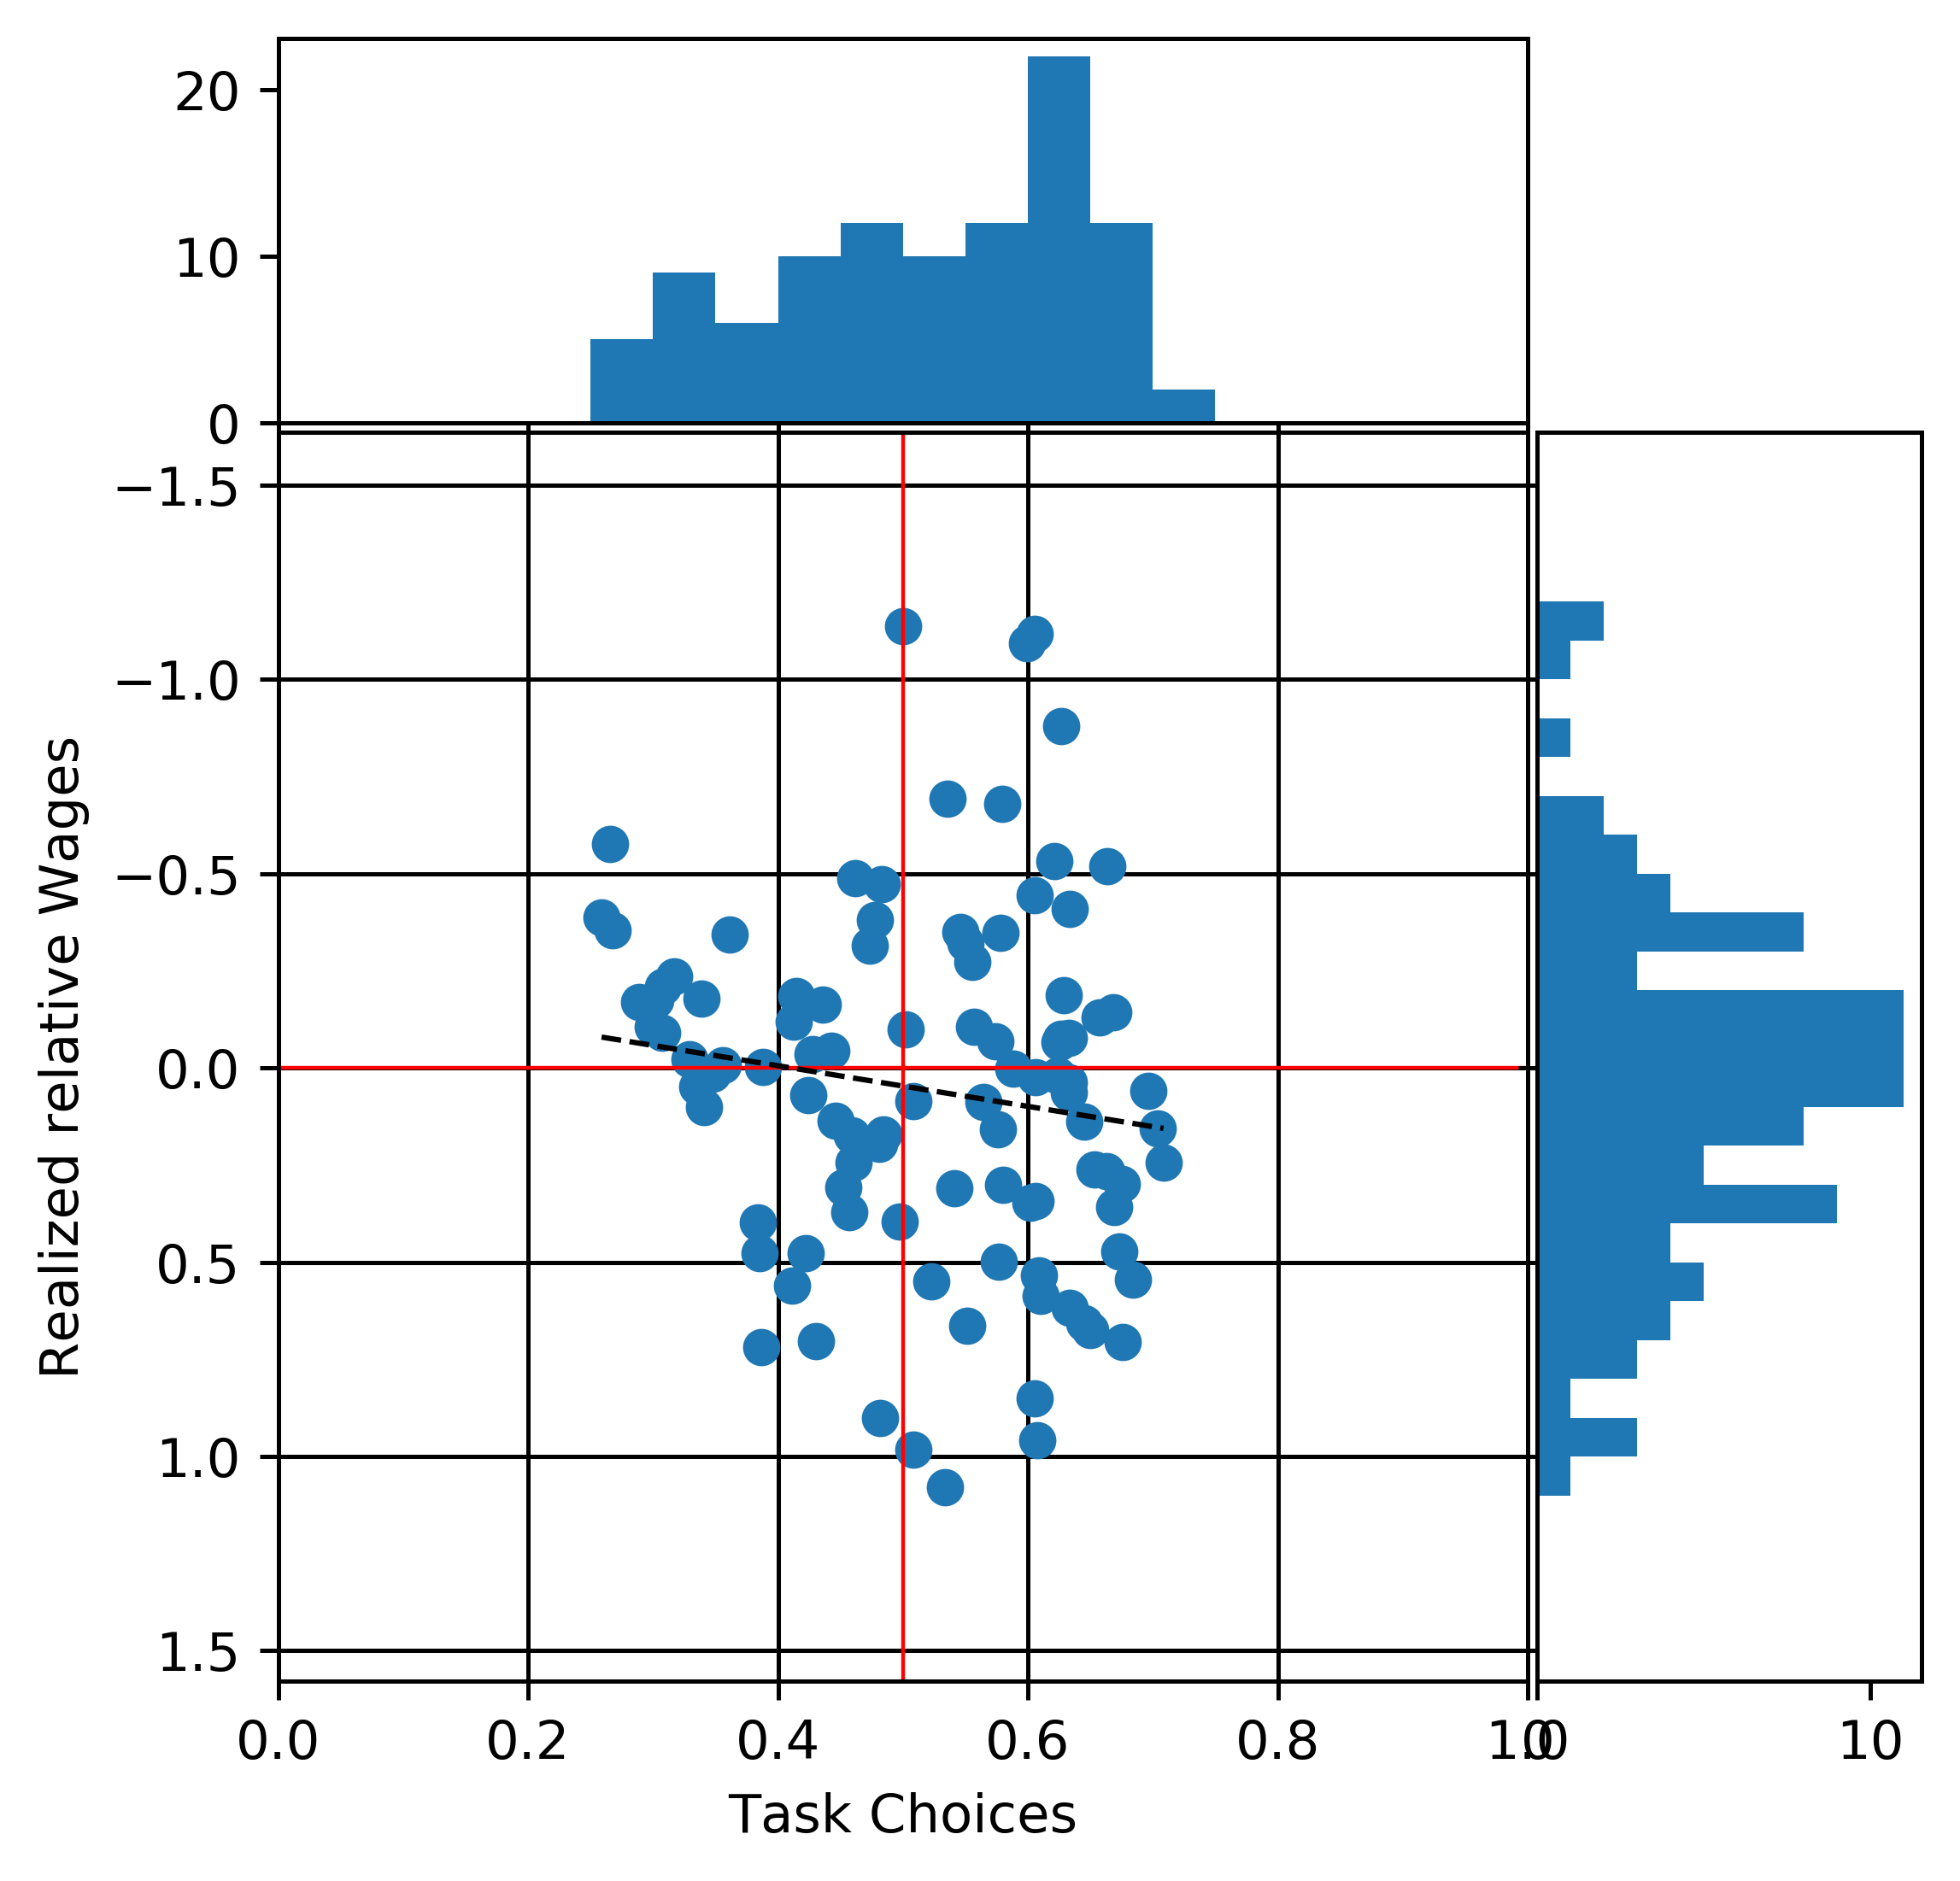
\includegraphics[scale=0.7]{./FIG/simulated_data.png} 
	\caption{Simulated data resulting from a data generating process that is specified as described in section \ref{sec:DGP}. This figure illustrates $N=100$ combinations of realized relative wages (i.e., sum of potential wages, weighted by task choices) and optimal task choices (i.e., the fraction of working time spent on task two) from the initial period $t=0$ in a scatter plot. Along each axis a histogram of the respective variable is plotted. The dashed line results from an OLS fit of realized relative wages (vertical axis) on optimal task choices (horizontal axis).}
	\label{fig:simulated_data}
\end{figure}
\\
Overall, the data generating process described in this section provides simulated data on task choices and realized wages for each period. From this, wage changes as well as adjustments in task choices can be calculated for the base period as well as a subsequent estimation period. Utilizing both, changes in task choices and realized wages, allows to draw inferences on the change in relative skill prices on which the data generating process is based. The next section shows the results of a Monte Carlo estimation of changes in skill prices relying on the identification strategy discussed in section \ref{sec:model_estimation} and using data that is generated by the process described in this section.

\FloatBarrier
\subsection{Monte Carlo Estimation of Skill Prices} \label{sec:MC_estimation}
% Following the identification strategy presented in section 2.4.:
%% use base period (without price changes) to estimate effects of changes in skill endowments as well as pentalty term 
%%% Present regression table: Show that I need to drop some regressors (multicol.), show that I capture most of the variance, show that estiates are highly significant.
%% use these estimations to calculate a "residual wage change" in estimation period, i.e., adjust wage changes for above mentioned effect
%% Regress residual wage change on mean lambda
%%% Show regression rslt: high significance, point estimate, R^2 should be relatively high in this model, too
% Present results from MC-Simulation (distribution of point estimates)
% Find reasons for bias in estimation: Why is my estimate too high? 
%% Do I not completely capture skill changes (same regressor)? 
%% Does dropping regressors in first step result in inappropriate estimators and, thus, biased estimations?
% overall: Model allows to obtain a close estimate of true price changes
%% Potentil problems and (1) Why they are not that relevant in real data and (2) what can be done to mitigate 
This section presents the results of a Monte Carlo estimation of changes in skill prices and serves as a proof of concept of the model presented in section \ref{sec:tractable-model-of-cont-task-choice} of this thesis, particularly of the estimation strategy discussed in section \ref{sec:model_estimation}. For this purpose it relies on data generated in the process described in previous section.
\\
The estimation of skill prices consists of three steps: First, it uses a base period to estimate the effects of skill accumulation and changes in the penalty term in the absence of changes in skill prices. This allows for second, adjusting observed wage changes of a subsequent period for these previously estimated effects. Finally, changes in skill prices are estimated based on these residual wage changes in a third step. Each of these steps is repeated $M=1000$ times in a Monte Carlo estimation, each time considering data on $N=100$ simulated individuals.
\\
In the particular model discussed in this work both, changes in skills and changes in the penalty term from $t-1$ to $t$, depend on task choices $\lambda_{i,t-1}^*$ and $\lambda_{i,t}^*$. This can be seen from equation (\ref{eq:wage_change}). Specifically, the effect of skill accumulation depends on the mean task choice of both periods, $\bar{\lambda}_{i,t}^*$. The change in penalty term, however, results as a polynomial of degree $\phi$ of these optimal task choices. A derivation of this result can be seen in appendix \ref{app:derive_changes_penalty_term}. In the setting of the data generating process that is used in this simulation study, it is assumed that $\phi = 2$. In this case, changes in the penalty term can be shown to be equivalent to the expression in equation (\ref{eq:changes_in_penalty}) below as shown in appendix \ref{app:derive_changes_penalty_term}. Therefore, both $\lambda_{i,t-1}^*$ and $\lambda_{i,t}^*$ as well as their squared values need to be included in a regression model to capture changes in skill endowments and penalty terms.
\begin{equation}\label{eq:changes_in_penalty}
	\rho_{i}(\lambda_{i,t}^*) - \rho_{i}(\lambda_{i,t-1}^*) = \lambda_{i,t-1}^{*2} + \lambda_{i,t}^{*2} + 2b_i(\lambda_{i,t-1}^* + \lambda_{i,t}^*) 
\end{equation}
% Now find the model that is actually used in estimation
% Due to strong correlation of lmbs, I suspect i will have to drop some. So go check different specifications and see how they perform in 
% (a) modelling base period and 
% (b) adjusting in estimation period
In an estimation of skill accumulation and changes in the penalty term, however, not all of these regressors can be included due to their near perfect multicollinearity. Not only will each task choice be correlated with its square. In addition, optimal task choices of subsequent periods will be correlated in the theoretical framework presented in this thesis. This is for two reasons: First, optimal task choices (equation (\ref{eq:lmb_opt})) are a function of potential wages. Potential wages, in term, are modeled as the sum of log skills and log skill prices. By the assumption of skill accumulation as a learning by doing process, potential wages will correlate between periods and, thereby, optimal task choices will be correlated as well. Second, optimal task choices are a function of the allocation preferences $b_i$ which are modeled to be time invariant. Calculating the correlation coefficients between task choices in $t-1$ and $t$ as well as their squares for one of the Monte Carlo iterations reveals that, indeed, correlations are very close to one. A correlation heatmap can be found in figure \ref{fig:corr_heatmap} of appendix \ref{app:tables_and_figures}.
\\
In order to avoid this multicollinearity, only task choices of either period $t-1$ or $t$ can be included as regressors. As seen from the estimation results in tables \ref{tab:base_period_regression_rlst_t-1} and \ref{tab:base_period_regression_rlst_t} (appendix \ref{app:tables_and_figures}), both of these estimation specifications appear to fit the simulation data well with an adjusted $R^2$ of 0.999 in either case. Each iteration of the Monte Carlo estimation is based on $N=100$ simulated observations. While this number is small enough to keep the computational load low, the resulting estimates have small standard deviations and high significance ($p<0.001$ for both estimates).
\\
Given there is an adjustment in task choices between periods, by construction the mean task choice lies in between the task choices in $t-1$ and $t$. This implies that dropping task choices in $t-1$ or $t$ in the estimation of skill accumulation and changes in the penalty term in the base period increases, or respectively, decreases the estimates. Consequently, estimated skill accumulation and changes in the penalty term will be biased. Therefore, both specifications will be considered in the following. In each of the $M=1000$ iterations of this Monte Carlo estimation, changes in skills and penalty term in the base period are estimated, once including task choices from $t-1$ and once from $t$. After that, wage changes of the subsequent time period are adjusted for the product of the estimated coefficient from the base period and the estimation period's task choices. Again, both possible setups are considered in this adjustment. Resulting residual wage changes are the basis of the estimation of changes in skill prices. 
\\
\begin{figure}[!htbp]
	\centering
	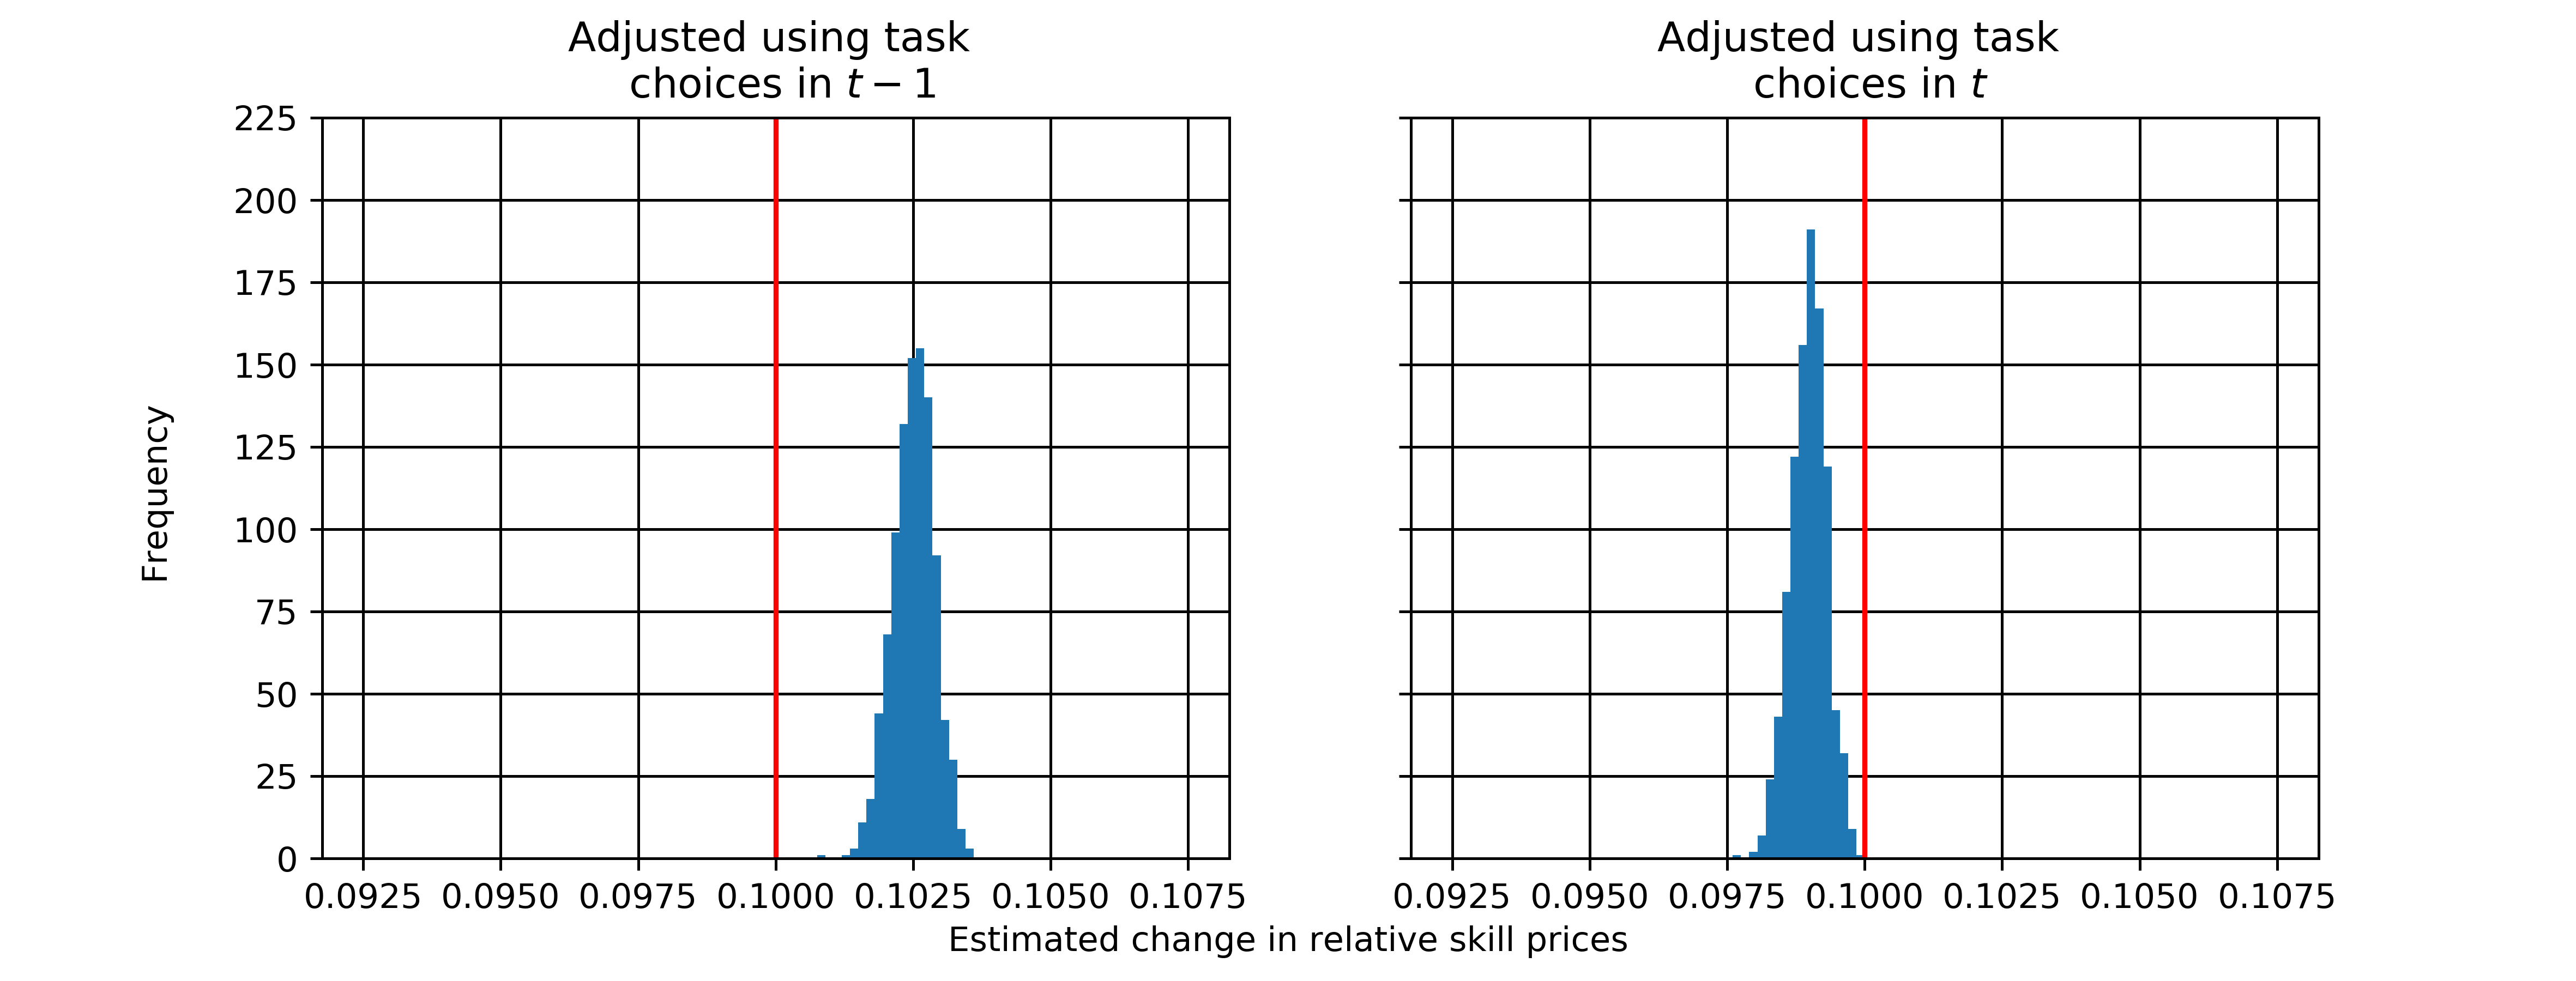
\includegraphics[scale=0.7]{../FIG/MC_estimation_rslt.png} 
	\caption{Histogram of the result of $M=1000$ Monte Carlo estimations of changes in relative skill prices. The true price changed used in the data generating process is $0.1$. Wage changes of the estimation period are adjusted for skill accumulation and changes in the penalty term. In the left panel, this adjustment uses task choices in $t-1$, in the right panel it uses task choices in $t$.}
	\label{fig:MC_est_rslt}
\end{figure}
Figure \ref{fig:MC_est_rslt} presents histograms of the results of the Monte Carlo estimation. The left panel presents the results from a setting where wage changes are adjusted based on an estimation that includes task choices from $t-1$. The panel on the right hand side results from a setting where this adjustment is based on task choices in $t$. Estimation results reveal to be noticeably biased in both panels. In the left panel estimation results have a positive bias, i.e. changes in relative wages are overestimated by up to approximately $0.5$ percentage points. Put into perspective with the true change in relative skill prices of $10 \%$, this corresponds to an overestimation in the order of magnitude of $5 \%$. In the right panel the opposite can be seen: changes in relative prices are underestimated. The estimation error is slightly smaller in this case and amounts up to circa $0.25$ percentage points. This corresponds to a relative deviation of $2.5 \%$. The true change in relative price changes ($0.1,$ indicated with the red vertical line) lies in between the estimation results based on adjustments using task choices in $t-1$ and the results based on adjustments using task choices in $t$.
\\
As argued above, a biased estimation result is to be expected as task choices of only one point in time can be included in the estimation of skill accumulation and changes in the penalty term. This leads to a biased estimation of these effects and, thus, either an under- or over correction of wage changes in the estimation period for changes in skill endowments and penalty. An accurate estimation of changes in relative skill prices can only result in a setting where task choices of both points in time, $t-1$ and $t$, are included. This specification, however, suffers from near perfect multicollinearity.
\end{document}